\pagestyle{fancy}

\begin{abstract}
The HIVE AURC Avionics (Data Analytics and Verification) capstone project was formed as part of RMIT HIVE's endeavours to compete in the 2024 Australian Universities Rocket Competition. Participants in this project acted as a part of the Aurora V avionics team, with the focus on developing systems for data analytics on the rocket, including the firmware implementation for real time processing and communications of data during flight, as well as avionics systems testing for verification.
\end{abstract}

\section{Introduction}

\subsection{Background}
The Australian Universities Rocket Competition (AURC) is one of Australia’s competitions for university student teams to design, build, and launch high-powered model rockets. The AURC is organised to encourage students from across Australia to develop technical and project management skills in aerospace engineering. Participating teams are required to launch rockets to specific altitudes, either 10,000 feet or 30,000 feet while integrating payloads and avionics systems that can capture and transmit real-time flight data. 

The competition is a significant platform for enabling innovation in aerospace technology, particularly focusing on rocketry, avionics, and data analytics. Teams are evaluated not only on the rocket’s performance but also on their design, safety considerations, and the accuracy of data acquisition during flight. 

A key focus area for the Aurora rockets has been the development of a reliable avionics system capable of handling the demands of high-speed, high-altitude flights. The Aurora V rocket, designed for the 2024 AURC, was expected to reach an apogee of 10,000 feet and relied on a custom avionics system for monitoring and controlling its flight. This competition not only pushes the technical boundaries of rocketry but also provides opportunities for students to engage in real-world engineering challenges. 

\begin{figure}[h]
    \begin{center}
        
\includegraphics[width=0.95\textwidth]{./img/subsystems_avionics.png}
    \end{center}
    \caption{Aurora Project subsystems}\label{fig:subsystems_avionics}
\end{figure}

The Aurora V team consisted of 30 students from various disciplines, including aerospace engineering, mechatronics, electronics, computer science and biomedical. The team is structured into several sub teams, each responsible for different aspects of the rocket’s design and performance. These sub teams include Avionics, Aerostructures, Ground Communications, Payload, Recovery and Aerobrakes -- as pictured in Figure~\ref{fig:subsystems_avionics}. The Data Analytics and Verification team, as a subset of the Avionics team, worked closely with these groups to ensure seamless integration of the custom hardware and firmware developed for flight monitoring and data analysis. This multidisciplinary collaboration enabled the Aurora V team to address complex engineering challenges from different engineering perspectives and deliver a rocket system that meets the requirements of the AURC competition. 

The Data Analytics and Verification team was responsible for not only gathering sensor data but also ensuring its accuracy through validation and real-time analysis. The team worked closely with the Avionics, Ground Communications, and Redundant Systems team, which was tasked with designing and building the custom hardware required for the avionics system. Meanwhile, the Data Analytics and Verification team focused on designing and implementing the custom firmware that enables sensor fusion, state estimation, telemetry, and communications between subsystems. 

This division of scope allowed for the ease of integration between the hardware and firmware, easing development across the board for the avionics team. Given the complexities involved in high-powered rocket flights, where the environment is constantly changing, this team was key in ensuring that flight data is accurate and can be used for both in-flight decisions and post-flight analysis. The team’s efforts are geared toward creating a more reliable and fault-tolerant avionics system that enhances the overall performance of the Aurora V rocket in the AURC. 

The final competition launch, initially planned to take place in Western Australia, was unfortunately cancelled due to logistical challenges, particularly the inability to secure rocket motors in time for the event. As a result, the AURC shifted to an online format, where teams would present their designs, systems, and findings rather than conducting a physical launch. In this modified competition format, the objective of the Data Analytics and Verification team has expanded to include providing comprehensive systems documentation and findings for future RMIT teams. 

These future teams will build on the groundwork laid by the current Aurora V team and aim to successfully compete in the next AURC and beyond by taking advantage of the avionics systems and data validation processes and findings developed during this project. 

\subsection{Problem Statement}
The primary challenge for the Data Analytics and Verification team was to design, implement, and validate data analytics and real-time verification processes for the Avionics system of the Aurora V rocket, which was expected to fly in the 2024 Australian Universities Rocket Competition (AURC). The avionics system, developed by the Avionics, Ground Communications, and Redundant Systems team, presents significant constraints, including limited processing power, memory, and communication bandwidth.

These limitations needed to be considered while ensuring the collection, logging, and real-time analysis of sensor data in-flight. Additionally, the Data Analytics and Verification team needed to ensure the accuracy of telemetry and state estimation to support critical flight functions such as the airbrake control system and recovery mechanisms. The challenge extended to testing these systems across multiple rocket iterations (Aurora I to V), ensuring that improvements were made with each launch.

\subsection{Project Deliverables}
For the major portion of this capstone, the objectives and deliverables were maintained. The following objectives and deliverables aim to delineate between objectives of the AURC and this capstone project team.

\begin{enumerate}
    \item \textbf{Data Capture and Logging Implementation}: Develop firmware to define sampling rates and intervals for sensor data capture and establish reliable logging formats for storage and later analysis.
    \item \textbf{Real-Time Data Processing}: Design algorithms for sensor fusion, incorporating multiple sensor inputs to produce accurate state estimation. Implement filtering techniques (e.g., Kalman filters) to reduce noise which is critical for the airbrake control system.
    \item \textbf{Post-Processing and Analysis}: Conduct post-flight statistical analysis to evaluate the performance of avionics systems. Detect deviations from expected behaviour, comparing raw sensor data with processed, fused data. Compare results against the Blue Raven flight computer to ensure accuracy.
    \item \textbf{Data Visualisation}: Develop tools to visualise data, generating graphs and charts that allow for clear interpretation of results. This also includes the potential for creating flight simulations based on collected data.
    \item \textbf{Data Validation}: Implement verification processes to assess the validity and integrity of captured data. This includes identifying and addressing data errors, hardware malfunctions, and inconsistencies.
\end{enumerate}

\subsection{Project Scope}
The Data Analytics and Verification team operates within the Avionics subsystem and focuses on the following key activities:

\begin{enumerate}
    \item \textbf{Software Development}: Design and develop firmware responsible for data collection, logging, and real-time processing. Post-processing involves visualising and analysing the collected data to detect anomalies and verify system performance.
    \item \textbf{Algorithm Development}: Research and implement sensor fusion, filtering (using techniques like the Kalman filter), and state estimation algorithms to ensure accurate in-flight data.
    \item \textbf{Testing and Validation}: Perform ground-based and in-flight testing (Aurora I to V) to validate the reliability and performance of the data analytics system. Each launch provides opportunities to refine the system based on feedback.
    \item \textbf{Iterative System Refinement}: Continuously refine the firmware and analysis algorithms based on data collected from each rocket iteration. This culminates in a competition-ready avionics system for Aurora V. Although the final Aurora V launch will not be part of the official competition, the findings and outcomes will contribute valuable insights for future students and teams, ensuring continuity and further development of the system for subsequent launches.
\end{enumerate}


\section{Literature Review}
\subsection{Data Analytics in Avionics}
\subsection{State Estimation Techniques}
\subsection{Real-Time Operating Systems (RTOS) in High Powered Rockets}
\subsection{Testing and Verification in Rocketry}

\subsubsection{Barometer and Vacuum Chamber Testing}
In rocketry, precise altitude measurement is essential for triggering key events, primarily the deployment of the recovery parachute. Barometric sensors, which measure air pressure to estimate altitude, are widely used for this purpose. To validate their performance under controlled conditions, vacuum chamber testing is a common method. This testing simulates the pressure changes a rocket would experience during ascent, allowing engineers to verify that the barometer accurately responds to varying altitudes and pressure changes. 

% TODO: citation
One study \cite{NAR-58} used a vacuum chamber to simulate altitudes ranging from 75 to 2100 meters, testing altimeters for their accuracy across these ranges. By correlating the chamber's pressure changes with expected altitude measurements, the study was able to validate both passive sensor monitoring and active sensor emulation methods. These tests are crucial to ensure that the barometers function reliably during flight and respond appropriately to dynamic environmental conditions, such as pressure fluctuations caused by wind or rapid altitude changes.
n rocketry, precise altitude measurement is essential for triggering key events, primarily the deployment of the recovery parachute. Barometric sensors, which measure air pressure to estimate altitude, are widely used for this purpose. To validate their performance under controlled conditions, vacuum chamber testing is a common method. This testing simulates the pressure changes a rocket would experience during ascent, allowing engineers to verify that the barometer accurately responds to varying altitudes and pressure changes. 

One study used a vacuum chamber to simulate altitudes ranging from 75 to 2100 meters, testing altimeters for their accuracy across these ranges. By correlating the chamber's pressure changes with expected altitude measurements, the study was able to validate both passive sensor monitoring and active sensor emulation methods. These tests are crucial to ensure that the barometers function reliably during flight and respond appropriately to dynamic environmental conditions, such as pressure fluctuations caused by wind or rapid altitude changes.

\subsubsection{Accelerometer and Gyroscope Testing}
In addition to the barometer, accelerometers and gyroscopes are key sensors used in rocketry to measure acceleration and angular velocity, respectively. These sensors provide important data for calculating the rocket's velocity, orientation, and trajectory. Ground testing of accelerometers typically involves placing the sensor in a controlled motion environment where its output can be compared against known values. For instance, flight motion simulators can recreate the conditions experienced during rocket flight, including G-forces and rapid directional changes. These setups allow engineers to calibrate the sensors, ensuring that their outputs remain accurate under high stress conditions​  

Inertial Measurement Units (IMUs), which combine accelerometers and gyroscopes, are also extensively tested in rocketry. These tests often involve multi-axis rate tables, which can simulate complex flight dynamics in multiple directions. Testing these systems helps in detecting sensor biases, misalignments, and nonlinearities.  The calibration process ensures that IMUs can accurately capture data that will be used for flight control and telemetry​.  

\subsubsection{General Testing in Rocketry}
% TODO citation
Beyond sensor-specific tests, rocket avionics systems undergo extensive testing to validate their performance under the high-stress environments experienced during flight. These systems must reliably operate under extreme conditions, such as high G-forces, vibrations, and rapid velocity changes. Ground-based tests are critical for identifying potential system failures before launch. One common approach is telemetry reliability testing, which ensures that real-time data transmission remains uninterrupted, even when the rocket reaches high speeds and altitudes. This process often uses radio frequencies, such as Xbee modules, to transmit data between the rocket and the ground station \cite{rocket_telemetry}.

One technique used is Hardware-in-the-Loop (HIL) simulations, to validate avionics systems in controlled environments. HIL simulations integrate the rocket's actual hardware, such as flight computers or controllers, with simulated inputs and outputs to replicate real flight conditions without exposing the rocket to the physical stresses of an actual launch. This method allows engineers to subject the system to various scenarios, including fault injection tests where simulated sensor failures or unexpected conditions are introduced to test the system’s resilience. For example, by using HIL simulation, engineers can test the rocket's response to potential sensor failures during flight. These simulations help in understanding how the avionics system would behave in nominal and off-nominal situations, such as when a sensor provides erroneous data or fails completely. In rocketry, this is particularly useful in identifying vulnerabilities that could lead to major failures. Additionally, precise calibration of the telemetry and control systems through HIL simulation ensures repeatability and consistency in the rocket's performance.

\section{Implementation and Design Justification}
\subsection{Aurora I and II}
Due to delays in hardware availability from vendors, the Aurora I avionics system was constructed using a minimalistic or "bare bones" design, incorporating only the most essential components that were readily available. Despite the limitations, the Aurora I system still enabled the team to test critical functionalities, such as sensor data capture and storage on flash memory. Although it did not meet the original Aurora I design goals, the system provided a valuable opportunity for the team to develop fundamental capabilities, which were pivotal in guiding the design of future systems, particularly for Aurora III. 

The avionics design for Aurora I primarily focused on creating a foundational framework for gathering and storing flight data. It served as a proof of concept for using custom electronics with an Arduino-based system for data logging and sensor integration. Despite the absence of more advanced features such as real time telemetry, the system gathered preliminary flight data that informed later iterations of the rocket's avionics system and provided real world data to formulate state estimations techniques.  

\subsubsection{Avionics Design Overview}
The Aurora I avionics system consisted of two main components:

\begin{itemize}
    \item \textbf{Commercial Off-The-Shelf (COTS) Blue Raven Flight Computers}: These were responsible for activating the drogue and main parachutes for recovery. Additionally, they recorded flight data, which was used for post-flight analysis.
    \item \textbf{Custom Avionics Board}: Built on a perfboard, this board housed an Arduino Nano microcontroller and several sensors, including an accelerometer, barometer, gyroscope, and magnetometer. These sensors provided data on the rocket's altitude, orientation, and velocity, all of which were essential for assessing flight dynamics. The Arduino Nano controlled data acquisition and storage, while a SerialFlash module was used to store sensor data onboard for later retrieval.
\end{itemize}

Key objectives of the Aurora I design were to:

\begin{itemize}
    \item Gain practical experience with the COTS Blue Raven flight computers.
    \item Test various battery configurations, sensor data collection, and flash memory storage in flight conditions.
    \item Capture flight data for post-flight analysis to improve avionics design for subsequent iterations.
\end{itemize}

\subsubsection{Firmware Architecture}
The high-level flow chart provided under Appendix A depicts how the Aurora I avionics system captures and transmits data. The primary goal was to facilitate post-flight analysis and verification, aligning with the data collection intervals of the Blue Raven system (500 Hz high resolution and 50 Hz low resolution). Due to timing constraints as a result of lesser performant hardware for Aurora I, the high-resolution interval was elected to operate at 250 Hz to ensure all processes have adequate time to complete. Data logging was initiated by a launch event detected when vertical acceleration exceeds a pre-defined threshold (5g at present). During flight, raw sensor data was stored onboard in flash memory. 

\paragraph{High Resolution Data Capture}

The high resolution interval (250 Hz) focuses on data from an Inertial Measurement Unit (IMU), comprising accelerometer, gyroscope, and magnetometer sensors. This high sampling rate is used to accurately capture subtle changes in aircraft motion and orientation. Raw data from sensor registers is combined with headers into data frames, stored in a buffer, and then written to flash memory. 

\paragraph{Low Resolution Data Capture and Transmission}

The low resolution interval (50 Hz) reads data from a barometer (pressure and temperature sensor) to determine altitude. Similar to the high resolution process, raw data is framed and temporarily stored in a buffer before writing to flash.  

\paragraph{Design Considerations and Implementation}

Alternative design approaches were considered, including a separate logging interval. However, the chosen design simplifies the system by consolidating flash writing and LoRa transmission into the low resolution interval. This streamlines data handling tasks while still meeting the core requirements. Although LoRa communications was included in the initial Aurora I software design, the hardware to support this was unavailable at the time due to delays in hardware delivery. As a result, testing for LoRa communications was organised to be implemented in Aurora II. 

\paragraph{Development Testing and Optimisation}

% TODO: include figure
During initial tests, it became apparent that there were significant delays in accessing sensor data, especially when handling the sensors at high frequencies. These delays are depicted in timing tests (Figure~\ref{fig:x}), where it was found that accessing data from the sensors was too slow to meet the system’s real-time data capture requirements. The primary cause of this issue was traced back to the overhead created by the sensor libraries, many of which included non-essential features that added unnecessary processing time. 

To address this, the team conducted a series of optimisation tests. These tests involved stripping back the libraries to include only the core functionalities necessary for flight operations. The library optimisations resulted in significantly reduced sensor access times, allowing the system to capture data within the designated intervals. These optimisations ensured that the avionics system closely replicates data and timing of the onboard Blue Ravens.

\subsubsection{Data Storage and Handling}

\subsection{Aurora III and IV}
\subsubsection{Avionics Design Overview}

\subsubsection{Firmware Architecture Design and implementation}

\begin{figure}[h]
  \centering
  \begin{tikzpicture}[
      node distance=0mm and 3mm,
      task/.style={rectangle, minimum height=6mm, rounded corners, draw=black!75, radius=5pt, anchor=west},
      tier/.style={rectangle, draw=black, minimum width=10cm, minimum height=1cm, anchor=west},
    ]
    \node (health) [task, xshift=2mm] {Health Monitor};
    \node (tierCRITICAL) [tier, label=left:{\color{red}CRITICAL}] {};

    \node (flash) [task, below=of health.south west, anchor=north west, yshift=-0.4cm] {Flash Write};
    \node (CANTx) [task, right=of flash] {CAN Tx};
    \node (tier-1) [tier, below=of tierCRITICAL, label=left:-1] {};

    \node (HDataAcq) [task, below=of flash.south west, anchor=north west, yshift=-0.4cm] {High Res Data Acquisition};
    \node (tier-2) [tier, below=of tier-1, label=left:-2] {};

    \node (LDataAcq) [task, below=of HDataAcq.south west, anchor=north west, yshift=-0.4cm] {Low Res Data Acquisition};
    \node (tier-3) [tier, below=of tier-2, label=left:-3] {};

    \node (state) [task, below=of LDataAcq.south west, anchor=north west, yshift=-0.4cm] {State Management};
    \node (tier-4) [tier, below=of tier-3, label=left:-4] {};

    \node (LoRa) [task, below=of state.south west, anchor=north west, yshift=-0.4cm] {LoRa Tx};
    \node (CANRx) [task, right=of LoRa] {CAN Rx};
    \node (tier-5) [tier, below=of tier-4, label=left:-5] {};

    \node (flashEN) [task, below=of LoRa.south west, anchor=north west, yshift=-0.4cm] {Flash enable};
    \node (idle) [tier, below=of tier-5, label=left:{\color{blue}Idle}] {};

    \draw[arrows = {Latex-Latex}] ([xshift=4mm]tierCRITICAL.north east)--node[label, right]{Priority}([xshift=4mm]idle.south east);
  \end{tikzpicture}
  \caption{Avionics RTOS task hierarchy}\label{fig:priority}
\end{figure}

\subsubsection{Data Processing and Verification}

\section{Testing and Validation}
\subsection{Sensor Testing}
\subsection{Vacuum Chamber testing}
The vacuum chamber test was designed to validate the accuracy of the barometer on the Aurora avionics board by comparing it the Blue Raven flight computer. The expected pressure readings at an apogee of 7,000 feet were targeted at approximately 78.36 kPa. This experiment simulated flight conditions and apogee by gradually reducing the pressure inside the vacuum chamber and monitoring both systems' performance. 

The setup of this experiment involved connecting the Pfeiffer vacuum gauge to the pump and chamber and placing both the barometer and Blue Raven inside. Calibration of the electronics was initiated, with the Blue Raven set to a ground test mode. Data collection started, and a launch event was triggered on the Blue Raven to mimic the rocket launch sequence. 

During the test, the vacuum pump gradually reduced the pressure, aiming for the target 78.36 kPa pressure. As the pressure approached this value, the system simulated apogee by maintaining the reduced pressure for a few seconds. To maintain this specific pressure for simulating apogee, the pressure leak was intentionally adjusted. This was achieved by fine-tuning the chamber’s pressure leak valve, allowing just enough air to enter the chamber to balance the amount of air being removed by the pump. By matching the air leak to the pump’s extraction rate, the pressure stabilised, holding at the desired level for a few seconds. The test ended with a slow depressurisation to simulate the descent back to ground pressure levels. 

% TODO: add appendix
Throughout the process, both data from the avionics system and the Blue Raven were collected for analysis. The key focus of the test was to validate the barometer’s ability to maintain accuracy throughout different pressure stages and verify the effectiveness of the calibration and apogee simulation process. Further experimental design details and risk assessments can be found under the Appendix~\ref{apdx:x}. 

\subsection{RTOS Task Verification}
\subsection{Ground Communications Testing}
\subsection{State Estimation Verification}

\section{Launch outcomes and Results}
\subsection{Aurora I}
\subsection{Aurora II}
\subsection{Aurora III}
\subsection{Aurora IV}
\subsection{Aurora V}

\section{Challenges}
\subsection{Time Constraints}
\subsection{Hardware Availability}
\subsection{Collaboration}
\subsection{Erroneous Data and Logic Errors}

\section{Recommendations and Future Work}
\subsection{Suggested Improvements}
\subsection{Further Development}

\section{Conclusions and Learning Outcomes}

\clearpage
\section{Acknowledgements}
As members of the 2024 AURC Aurora V Avionics team we wish to acknowledge our incredible capstone supervisor, Dr. Glenn Matthews, without whose invaluable support and guidance we likely would not have come as far in our endeavours as we have. 

Throughout the year Glenn has gone above and beyond with his involvement with the team, attending many of our launches and showing a level of support for his students and for the project greater than we have seen from any other academic. With his assistance we managed to overcome many obstacles and have learned much more than we could have expected.

\begin{figure}[h]
    \begin{center}
        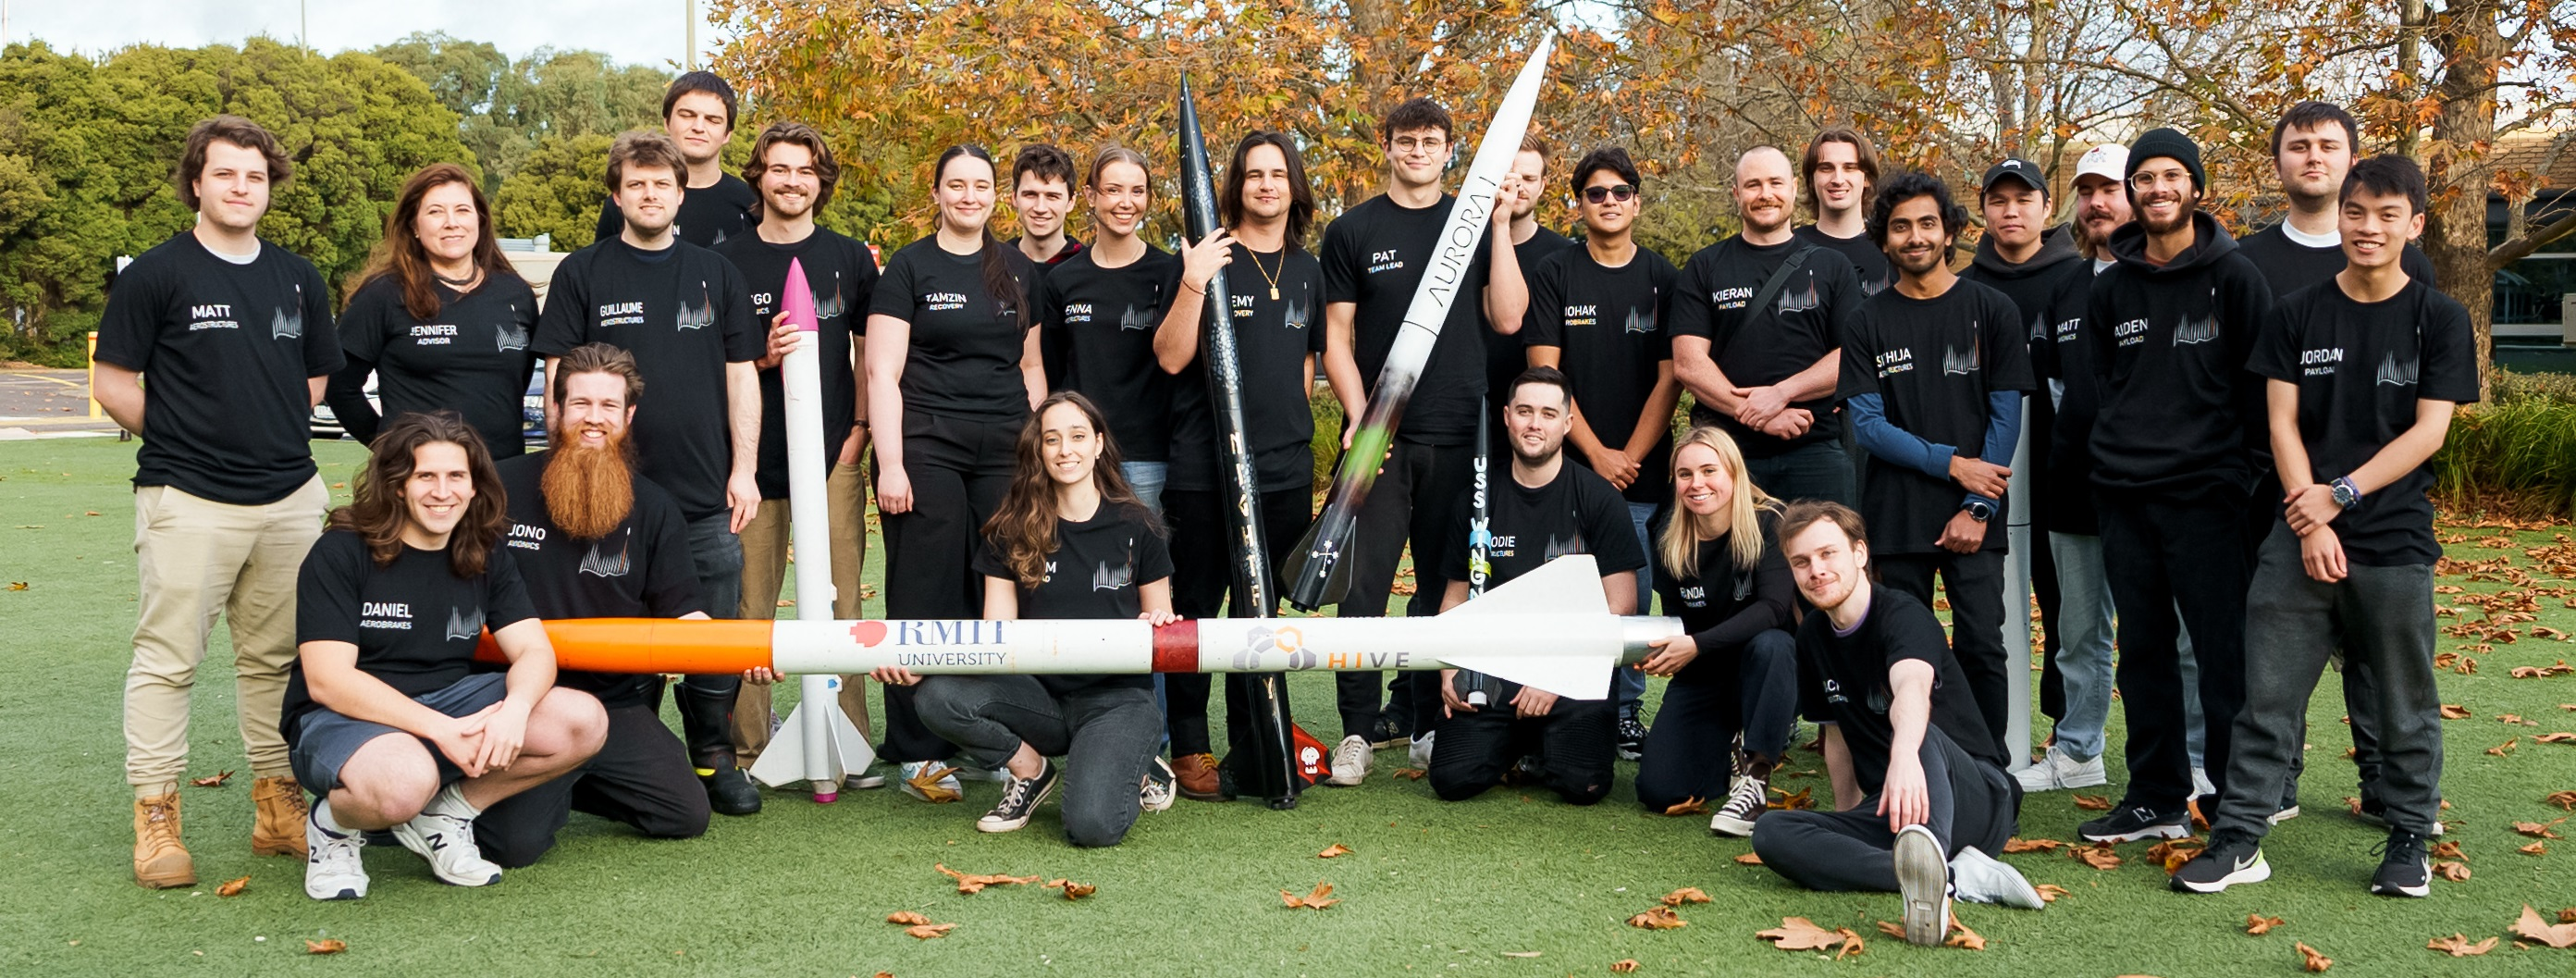
\includegraphics[width=\textwidth]{./img/aurora_team.jpg}
    \end{center}
    \caption{AURC Aurora V team 2024}\label{fig:aurora_team}
\end{figure}

We would also like to extend our gratitude to the greater Aurora team, for the amazing opportunity and experience this past year. We have come a long way since the beginning of this project, and through the ups and downs have managed to build and launch five rockets from the ground up. 

\hfill{}\textbf{Thank You}\hfill{}

\vfill{}\hfill{}Our rockets went brrr...
